\documentclass[12pt,a4paper]{article}
\usepackage{graphicx, booktabs, siunitx, amsmath, geometry, float}
\usepackage{subcaption}
\usepackage[backend=biber, style=ieee]{biblatex}
\addbibresource{references.bib}

\geometry{margin=2.5cm}
\title{Scanning Tunneling Microscopy Study of Highly Oriented Pyrolytic Graphite (HOPG)}
\author{Gregorio Jaca (U8L9B9), Peter Tallosy (K14WR1)}
\date{\today}

\begin{document}
\maketitle

\begin{abstract}
We used a Scanning Tunneling Microscope (STM) to investigate the surface of a Highly Oriented Pyrolytic Graphite (HOPG) sample. We characterized the instrument\'s performance and explored the atomic and electronic properties of the graphite surface. We investigated the effect of the vertical scanning range (z-limit) on resolution, measured the height of atomic steps, achieved atomic resolution to determine the lattice constant, and analyzed a Moiré superstructure to calculate the rotational angle between graphene layers. The measured lattice constant was 0.252 nm and the Moiré pattern indicated a twist angle of 1.09 degrees.

\end{abstract}

\section{Introduction}
The Scanning Tunneling Microscope (STM), invented by Gerd Binnig and Heinrich Rohrer in 1981, is a foundational tool in nanoscience, enabling the visualization and manipulation of surfaces at the atomic scale \cite{stm_manual}. It operates based on the quantum mechanical phenomenon of electron tunneling. When a sharp, conductive tip is brought within a few angstroms of a conductive sample, and a small bias voltage is applied, electrons can tunnel across the vacuum gap, generating a measurable tunneling current. This current is exponentially dependent on the tip-sample distance, providing the STM with its exceptional vertical sensitivity. The exponential dependance and a sharp tip ensures that (practically) all the current goes through a single point, the closest point of the tip to the sample. The quality of the tip can be ensured by the quality of the obtained images, making the calibration verification straightforward.

The goals of this lab are:
\begin{enumerate}
    \item To investigate the relationship between the vertical scanner range (z-limit) and the achievable vertical resolution.
    \item To measure the height of atomic steps on the HOPG surface and relate them to the graphene interlayer spacing.
    \item To achieve atomic resolution and determine the lattice constant of the graphite crystal.
    \item To analyze a Moiré pattern arising from twisted graphene layers and determine the corresponding rotation angle.
\end{enumerate}

\section{Theoretical Background}
\subsection{Tunneling Current}
In the constant current (topographic) mode, the STM feedback loop adjusts the vertical position (z) of the tip to maintain a constant tunneling current ($I_t$) as it scans across the surface (x,y). For small bias voltages ($U_t$), the tunneling current is proportional to the local density of states (LDOS) of the sample at the Fermi level ($E_F$) \cite{stm_manual}.
\begin{equation}
    I_t(r, U_t) \propto U_t \cdot \rho_{\text{sample}}(E = E_F, r)
\end{equation}
The resulting $z(x,y)$ map provides a convolution of the surface topography and its electronic structure.

\subsection{Moiré Effect}
When two periodic lattices are overlaid with a relative twist angle, a larger-period superstructure, known as a Moiré pattern, can emerge. For two stacked graphene layers with a lattice constant $d$ and a small twist angle $	heta$, the period of the Moiré pattern $D$ is given by:
\begin{equation}
    D = \frac{d}{2 \sin(\theta/2)}
    \label{eq:moire}
\end{equation}
This phenomenon allows for the precise determination of the twist angle between layers from a large-scale STM image.

\section{Experimental Methods}
The experiment was performed using a Veeco/DI Nanoscope 3 STM operating in ambient air. The scanning tip was mechanically cut from a Platinum-Iridium (Pt-Ir) wire. The quality of the tip was tested until a satisfactory one was found. We were careful in checking for tip degradation during the measuring, ensuring high quality images.

The STM was operated in constant current mode. Images were acquired using the Nanoscope software, with typical parameters of a bias voltage between 50 and 500 mV and a tunneling setpoint current between 500 pA and 2 nA. We investigated different parameter configurations for different measurements, always striving to get the best quality images, while protecting the tip from degradation. The acquired data was processed and analyzed using the Gwyddion software. Analysis steps included plane fitting to correct for sample tilt, row alignment to correct for scanner artifacts, and 2D Fast Fourier Transform (FFT) filtering to reduce noise in atomic-resolution images.

\section{Results and Discussion}

\subsection{Vertical Resolution vs. Z-limit}
The vertical resolution of the STM is limited by the 16-bit Digital-to-Analog Converter (DAC) that controls the z-piezo. The minimum vertical step size is determined by the total vertical range, or z-limit, according to: Resolution = $z_{\text{limit}} / 2^{16}$. We acquired images at different z-limit values to observe this effect.

\begin{figure}[H]
    \centering
    \begin{subfigure}[b]{0.48\linewidth}
        \centering
        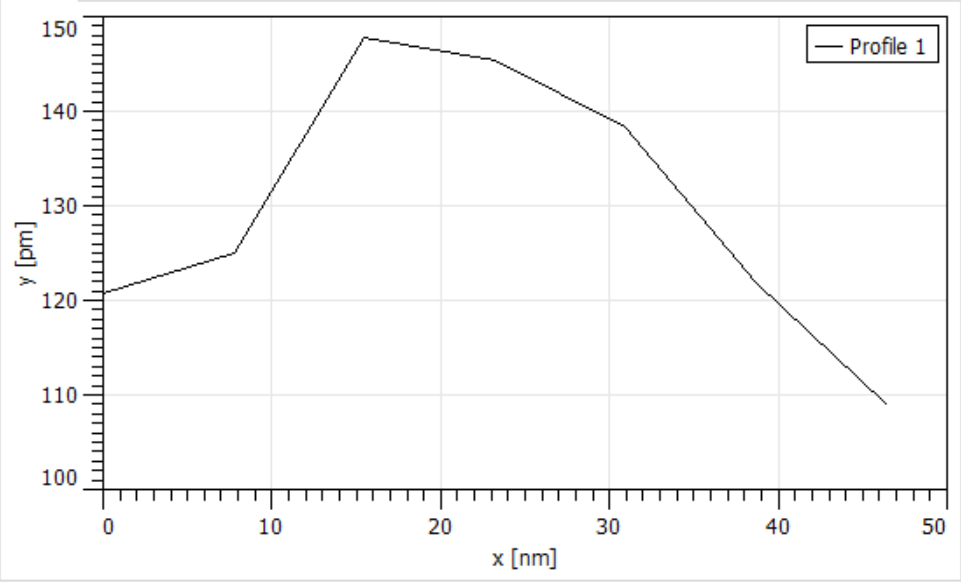
\includegraphics[width=\linewidth]{../data/tasks/1/2342nm.PNG}
        \caption{Image with a large z-limit (2342 nm).}
        \label{fig:high_z_limit_image}
    \end{subfigure}\hfill
    \begin{subfigure}[b]{0.48\linewidth}
        \centering
        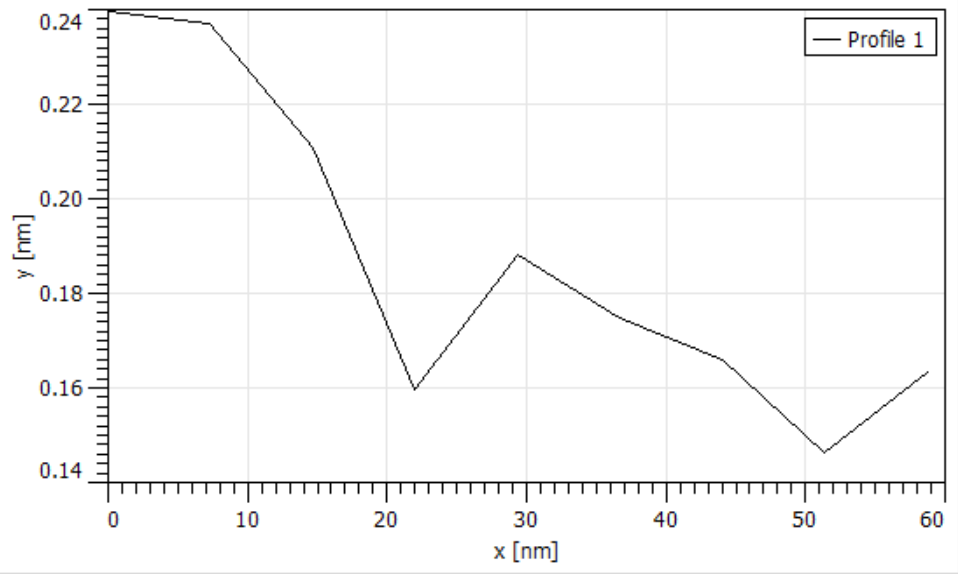
\includegraphics[width=\linewidth]{../data/tasks/1/500nm.PNG}
        \caption{Image with a small z-limit (500 nm).}
        \label{fig:low_z_limit_image}
    \end{subfigure}
    \caption{STM topography images of HOPG taken with different z-limit settings. A smaller z-limit provides lower noise and higher effective resolution.}
    \label{fig:z-limit}
\end{figure}
For a z-limit of 2342 nm, the theoretical resolution is \(2342 \text{ nm} / 2^{16} \approx 35.7 \text{ pm}\), while we obtained a resolution of \(\approx 42 \text{ pm}\). For a z-limit of 500 nm, it is \(500 \text{ nm} / 2^{16} \approx 7.6 \text{ pm}\) and we obtained a resolution of \(\approx 14 \text{ pm}\). While a smaller z-limit offers finer theoretical resolution, it also restricts the ability to track large topographic features. We found that a z-limit of 500 nm provided a good balance for locating atomic steps when operating in flat regions.

\subsection{Atomic Steps on HOPG}
The cleaved HOPG surface exhibits atomically flat terraces separated by steps. We located several of these steps and measured their heights using line profile analysis. We compare the heights with the literature value for the interlayer distance in graphite.

\begin{figure}[H]
    \centering
    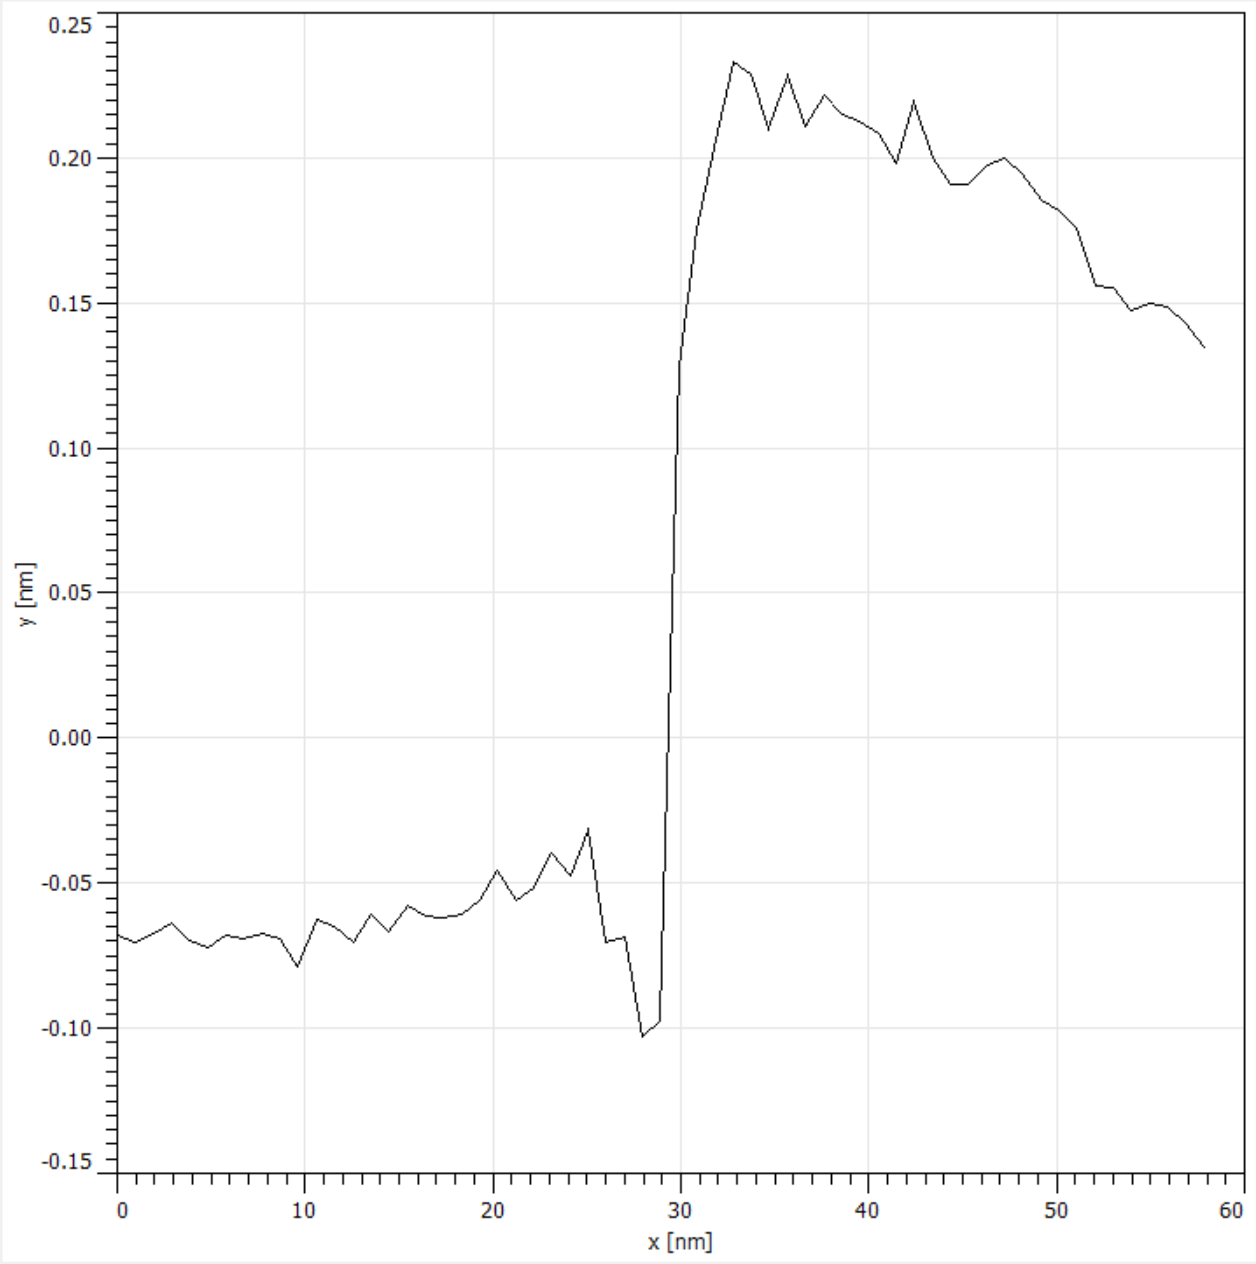
\includegraphics[width=0.7\linewidth]{../data/tasks/2/graph.PNG}
    \caption{STM image of HOPG showing atomic terraces, with a line profile indicating the height of a step.}
    \label{fig:step}
\end{figure}
The line profile shows a step height of approximately 0.33 nm (0.23 - (-0.10) nm). The known interlayer spacing for graphite is about 0.34 nm. Therefore, this step corresponds to N = $(0.33 \text{ nm} / 0.34 \text{ nm}) \approx 1$ layer of graphene.

\begin{figure}[H]
    \centering
    \begin{subfigure}[b]{0.48\linewidth}
        \centering
        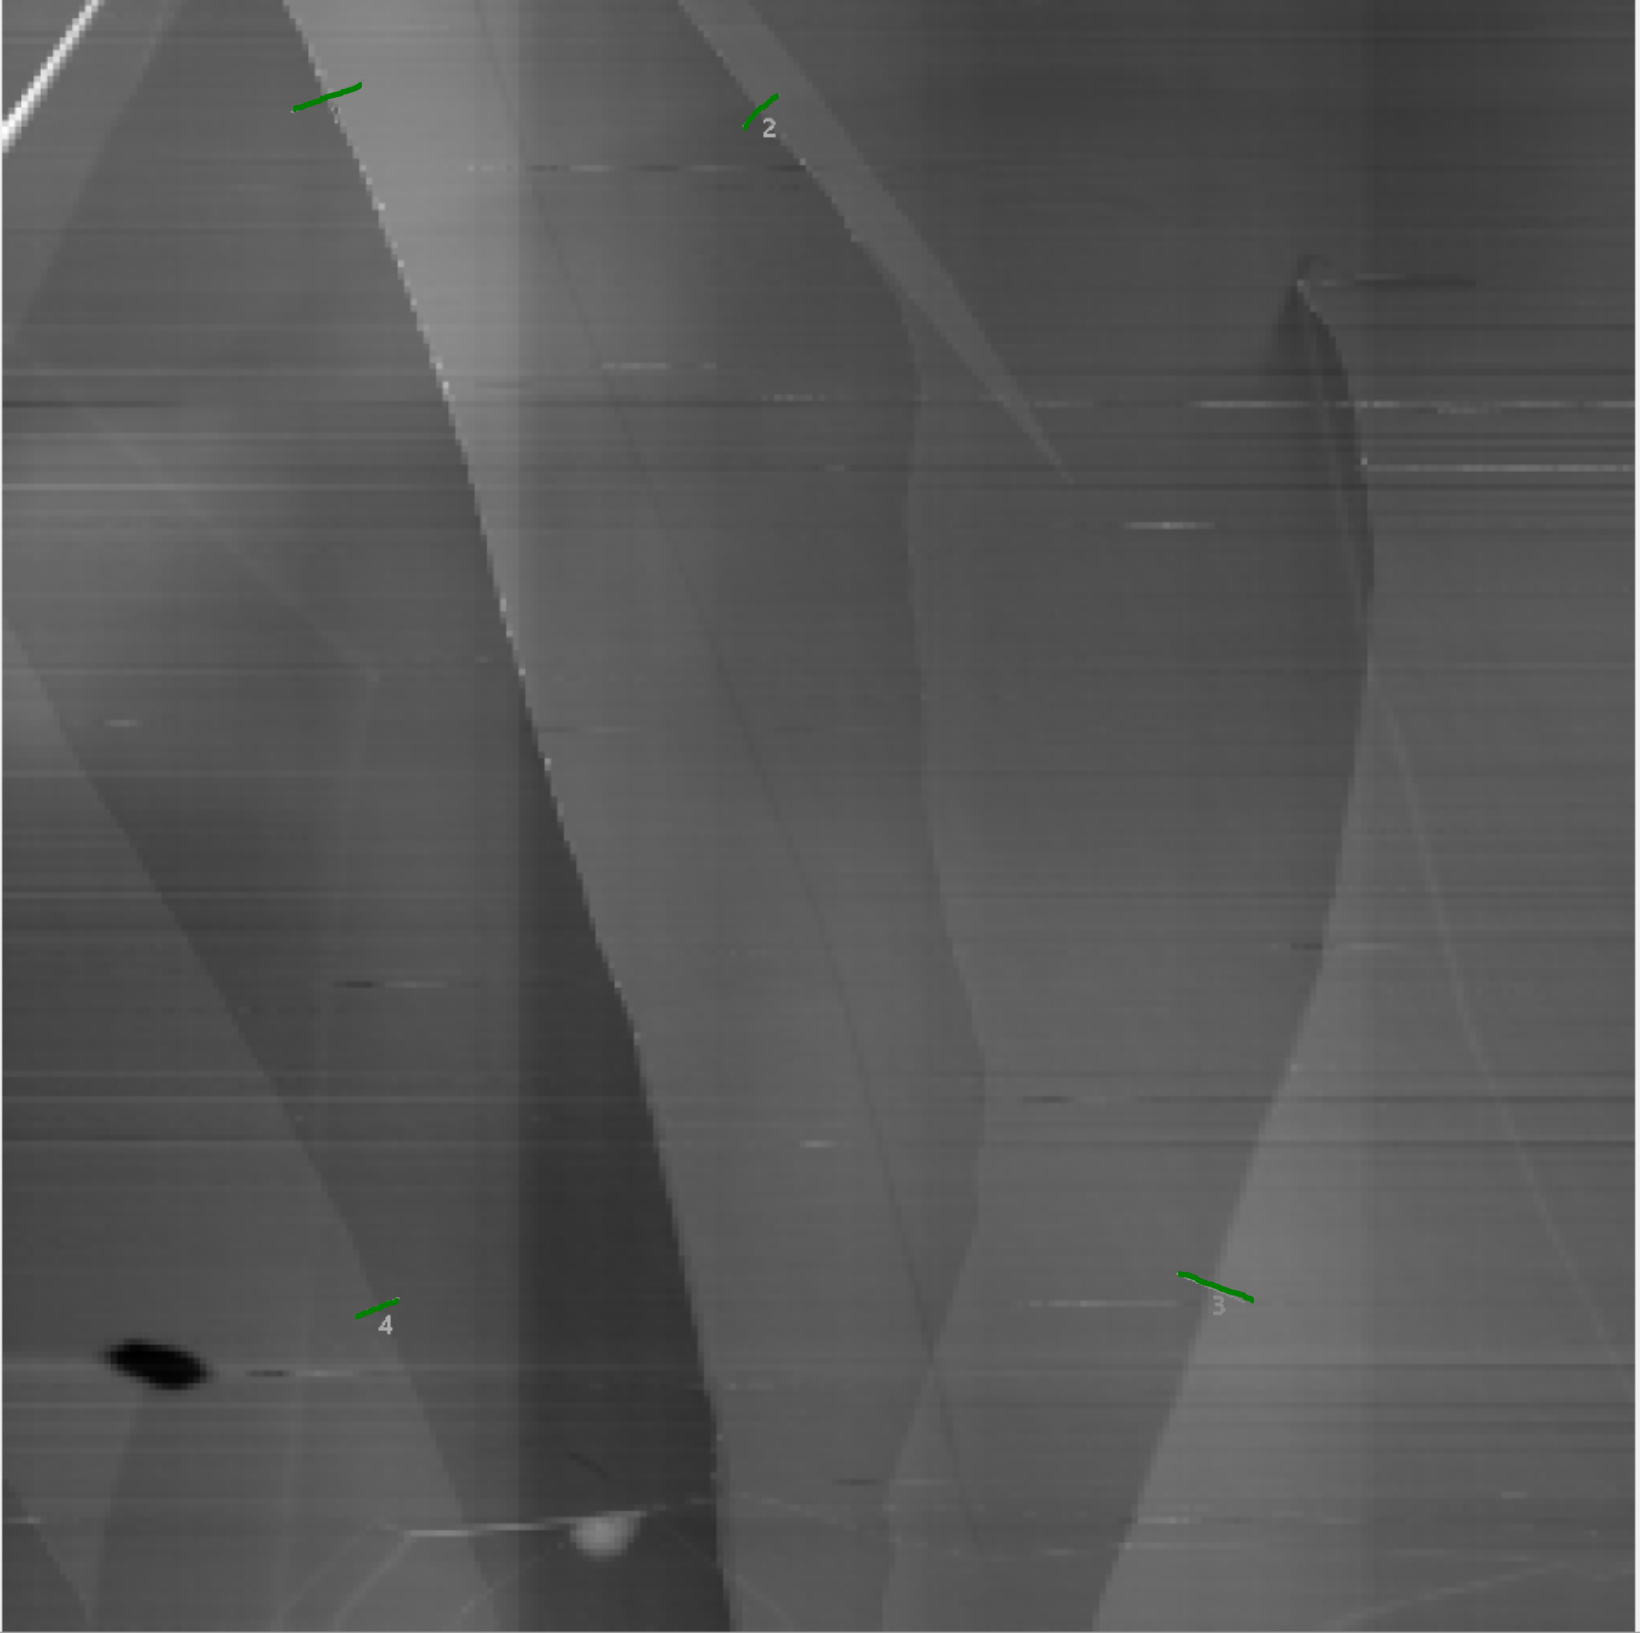
\includegraphics[width=\linewidth]{../data/tasks/1/original.PNG}
        \caption{Image of the graphite surface showing terraces.}
        \label{fig:terraces}
    \end{subfigure}\hfill
    \begin{subfigure}[b]{0.48\linewidth}
        \centering
        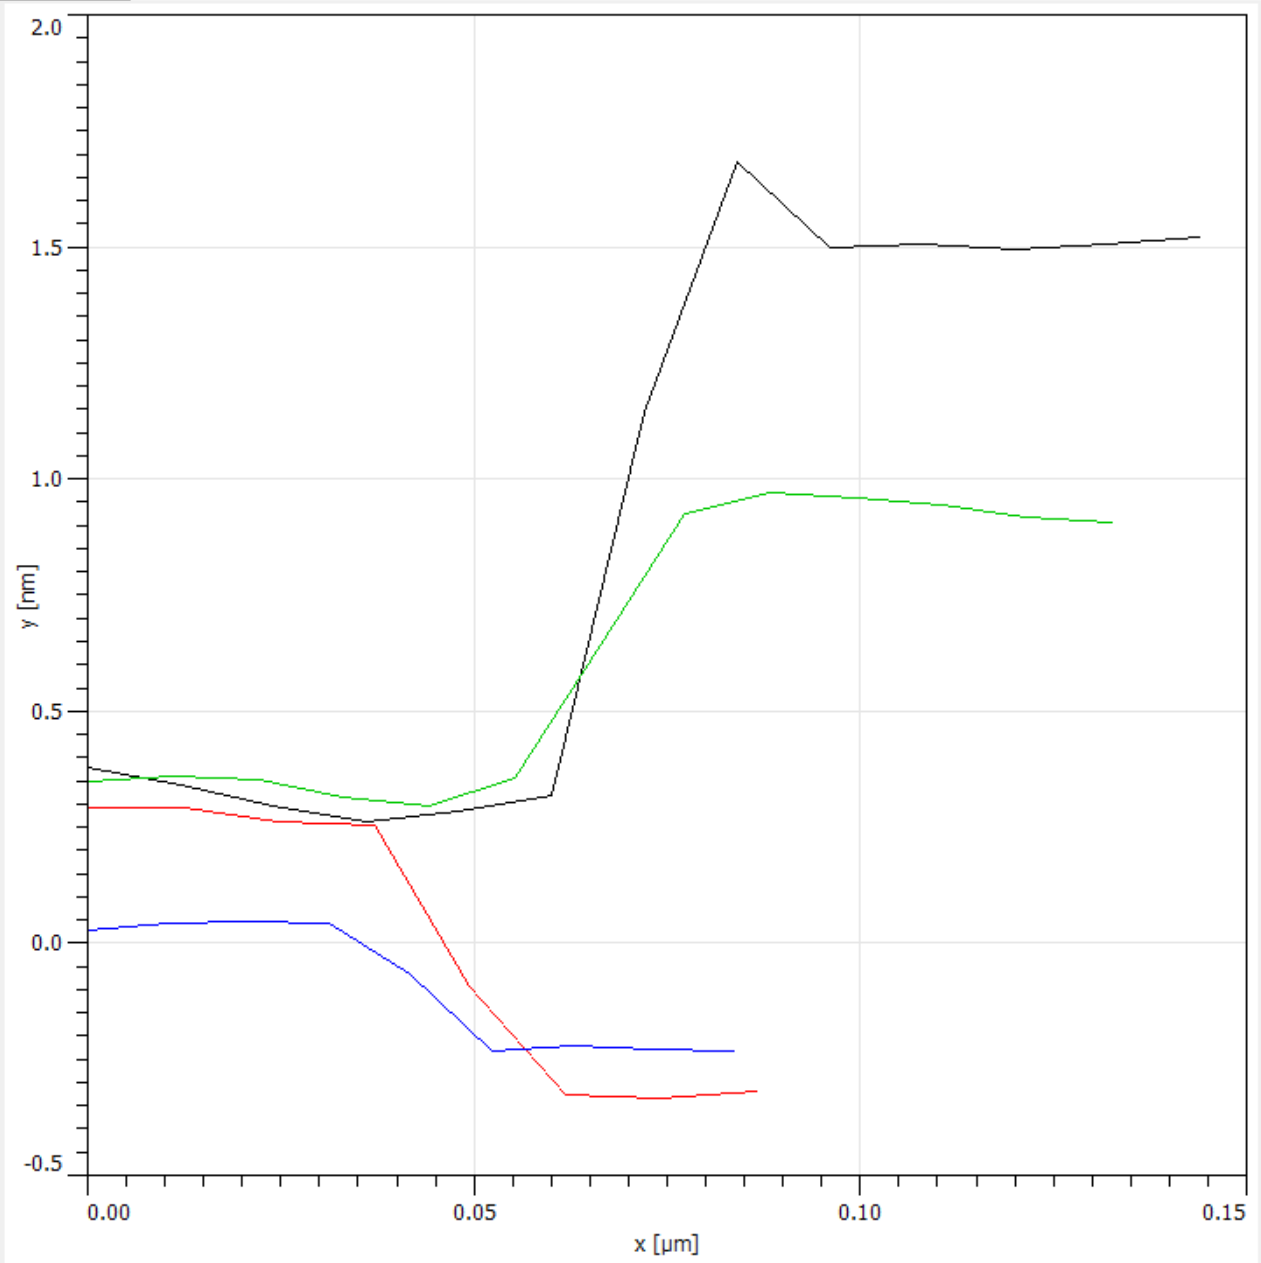
\includegraphics[width=\linewidth]{../data/tasks/1/Capture.PNG}
        \caption{Altitude profiles at several terrace boundaries.}
        \label{fig:altitude_profiles}
    \end{subfigure}
    \caption{STM topography images of HOPG showing terraces and altitude profiles. The profiles show single terrace steps of $\approx 0.34 \text{ nm}$ (green), and some multi-atom steps: two-layer (red and green) and four-layer (black).}
    \label{fig:terraces_and_profiles}
\end{figure}


\subsection{Atomic Resolution and Lattice Constant}


We scanned a small, flat area which was identified from a previous image, for which, as there were no terraces, we could safely reduce the surface-tip distance, by increasing the current setpoint value to 2.39 nA and reduced the Bisas voltage to 51.7 mV. After applying a 2D FFT filter to the atomically resolved scan, we observed the characteristic triangular pattern of atoms on the HOPG surface. This appearance, rather than the expected hexagonal honeycomb structure, arises because the STM primarily images only one of the two types of carbon atoms (A-site vs. B-site) due to differences in the local density of states.

To determine the lattice constant, we performed a line profile analysis on the filtered image, as shown in Figure \ref{fig:atomic-res}. The profile measures the periodicity of the atomic lattice along a specific direction.

\begin{figure}[H]
    \centering
    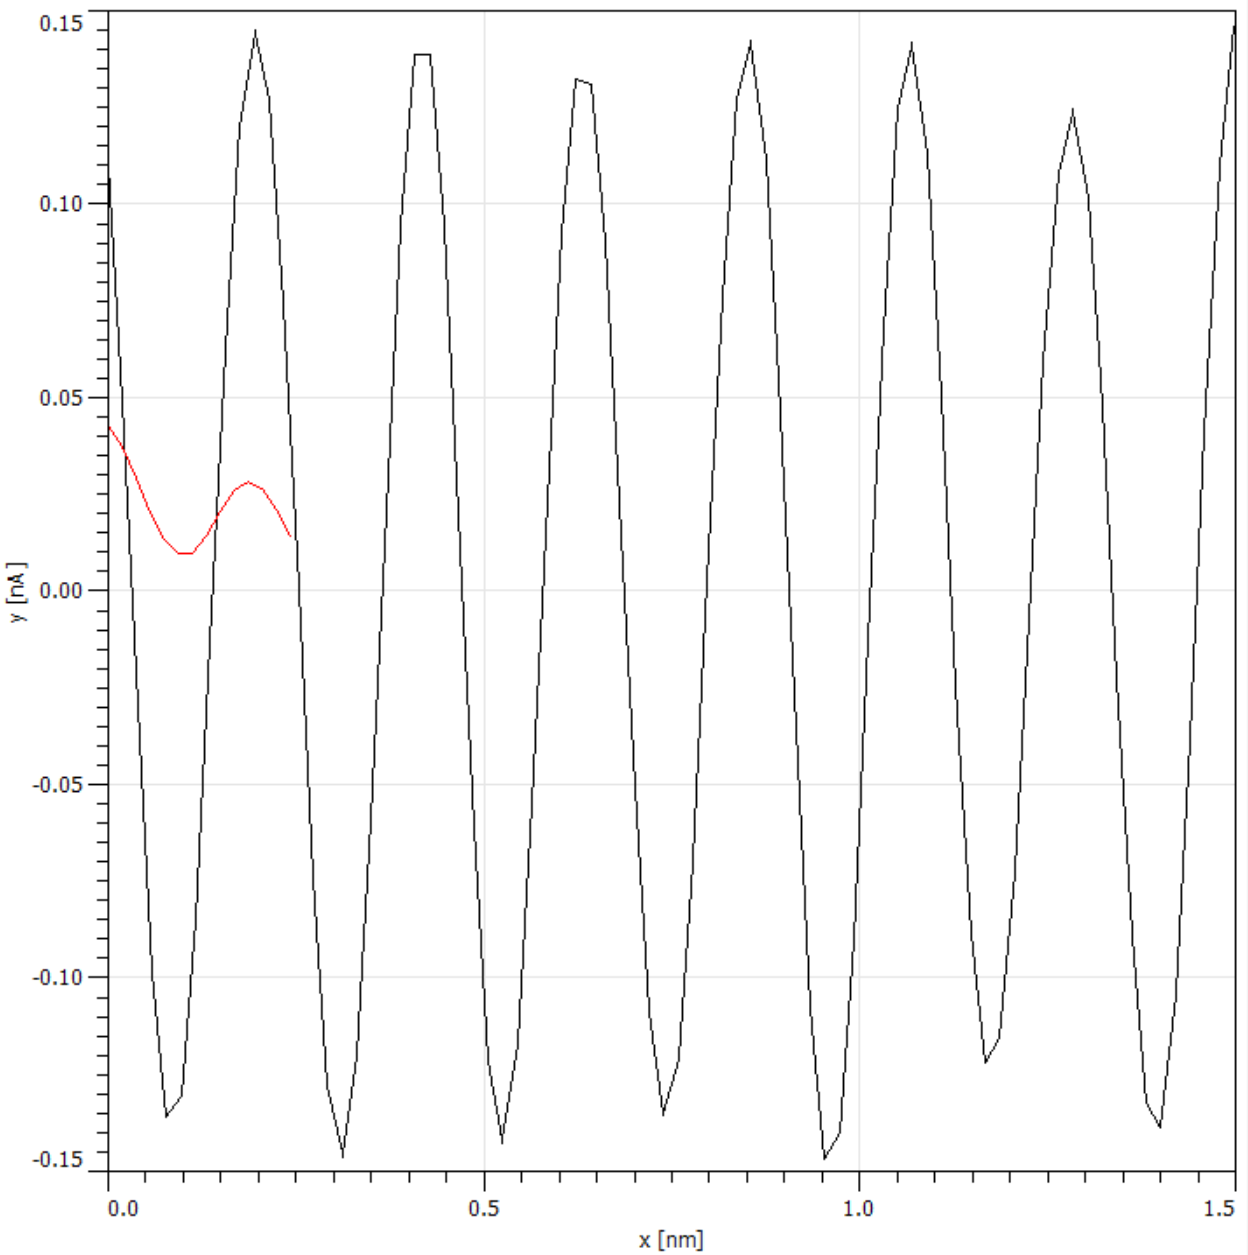
\includegraphics[width=0.8\linewidth]{../data/tasks/3/intermolecular_distance.PNG}
    \caption{Line profile taken across the atomically resolved and filtered STM image of the HOPG surface. The plot shows the tunneling current variation, with the peaks corresponding to the positions of the imaged carbon atoms. The periodicity directly relates to the lattice constant.}
    \label{fig:atomic-res}
\end{figure}

From the line profile, the distance between adjacent peaks was measured to be approximately 0.252 nm. This corresponds to the lattice constant 'a' of the hexagonal lattice. The theoretical value is a = 0.246 nm. Measurements along the three equivalent lattice directions showed minor variations, consistent with the expected effects of thermal drift. Discrepancies can arise from thermal drift and piezo scanner calibration.

\subsection{Moiré Pattern and Layer Rotation Angle}
In one region of the sample, we observed a Moiré superstructure, indicating the presence of at least two graphene layers with a rotational mismatch. The image obtained remarkably shows both the atomic-resolution graphite lattice and the larger Moiré superstructure simultaneously.

\begin{figure}[H]
    \centering
    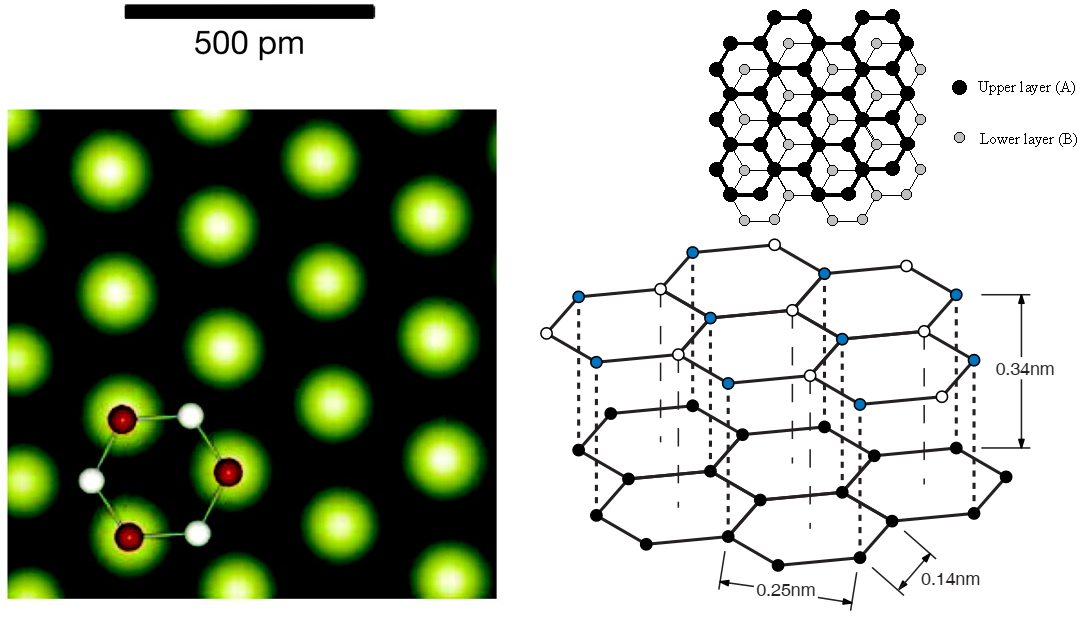
\includegraphics[width=0.6\linewidth]{../data/gergo_data/hopg.png}
    \caption{Large-scale STM image showing a Moiré pattern on the HOPG surface, caused by a rotational twist between graphene layers.}
    \label{fig:moire}
\end{figure}

We measured the period of the Moiré pattern, D, to be 12.89 nm. Using Equation \ref{eq:moire} and the theoretical graphene lattice constant d = 0.246 nm, we calculated the twist angle $\theta$ to be 1.09 degrees.

\begin{figure}[H]
    \centering
    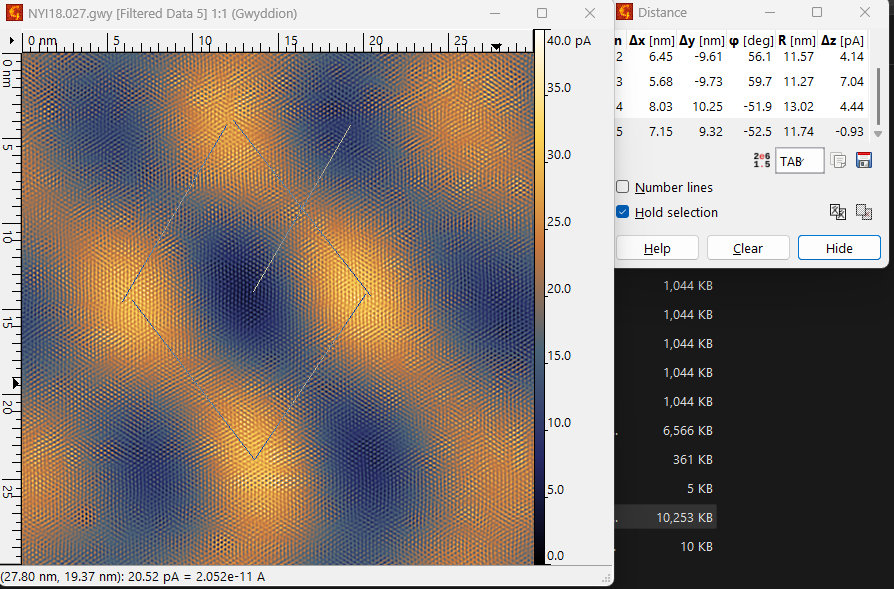
\includegraphics[width=0.7\linewidth]{../data/tasks/4/moire_with_dist.png}
    \caption{Measurement of Moiré pattern D}
    \label{fig:moire_dist}
\end{figure}

\section{Conclusion}

In this experiment, we successfully used a scanning tunneling microscope to explore the surface of HOPG. We characterized the instrument\'s vertical resolution and demonstrated the trade-offs involved in selecting the z-limit. We measured the heights of atomic steps, confirming their correspondence to integer multiples of the graphene layer spacing. Furthermore, we achieved atomic resolution, observing the characteristic triangular pattern of the graphite surface and determined the lattice constant to be 0.252 nm.
Finally, we analyzed a Moiré pattern to determine the twist angle between graphene layers to be 1.09 degrees. Potential sources of error in the measurements include thermal drift, acoustic vibrations, and the quality of the scanning tip.

\printbibliography

\section*{Appendix: Experimental Parameters}
\subsection*{Atomic Resolution Scan Parameters}
\begin{figure}[H]
    \centering
    \begin{minipage}[t]{0.48\linewidth}
        \centering
        \textbf{Scan Controls}
        \begin{tabular}{|l|l|}
        \hline
        Scan size: & \SI{10.0}{\nano\meter} \\
        X offset: & \SI{4.97}{\micro\meter} \\
        Y offset: & \SI{-44.0}{\nano\meter} \\
        Scan angle: & \SI{0.00}{\degree} \\
        Scan rate: & \SI{30.5}{\hertz} \\
        Tip velocity: & \SI{0.610}{\micro\meter\per\second} \\
        Samples/line: & 512 \\
        \hline
        \end{tabular}
        
        \vspace{0.5cm}
        
        \textbf{Other Controls}
        \begin{tabular}{|l|l|}
        \hline
        Microscope mode: & STM \\
        Z limit: & \SI{357.5}{\nano\meter} \\
        Units: & Metric \\
        Color table: & 12 \\
        Serial number: & 5342EV \\
        \hline
        \end{tabular}
    \end{minipage}\hfill
    \begin{minipage}[t]{0.48\linewidth}
        \centering
        \textbf{Feedback Controls}
        \begin{tabular}{|l|l|}
        \hline
        SPM feedback: & Log \\
        Current setpoint: & \SI{2.390}{\nano\ampere} \\
        Integral gain: & 0.5038 \\
        Proportional gain: & 1.581 \\
        Bias: & \SI{51.71}{\milli\volt} \\
        \hline
        \end{tabular}
        
        \vspace{0.5cm}
        
        \textbf{Channel 1}
        \begin{tabular}{|l|l|}
        \hline
        Data type: & Height \\
        Data scale: & \SI{100.0}{\pico\meter} \\
        Line direction: & Trace \\
        Realtime planefit: & Line \\
        Offline planefit: & Full \\
        \hline
        \end{tabular}
        
        \vspace{0.5cm}
        
        \textbf{Channel 2}
        \begin{tabular}{|l|l|}
        \hline
        Data type: & Current \\
        Data scale: & \SI{500.0}{\pico\ampere} \\
        Line direction: & Retrace \\
        Realtime planefit: & Line \\
        Offline planefit: & Full \\
        \hline
        \end{tabular}
    \end{minipage}
\end{figure}

\subsection*{Moiré Pattern Scan Parameters}
\begin{figure}[H]
    \centering
    \begin{minipage}[t]{0.48\linewidth}
        \centering
        \textbf{Scan Controls}
        \begin{tabular}{|l|l|}
        \hline
        Scan size: & \SI{500}{\nano\meter} \\
        X offset: & \SI{4.86}{\micro\meter} \\
        Y offset: & \SI{-17.1}{\nano\meter} \\
        Scan angle: & \SI{0.00}{\degree} \\
        Scan rate: & \SI{1.00}{\hertz} \\
        Tip velocity: & \SI{1.00}{\micro\meter\per\second} \\
        Samples/line: & 512 \\
        \hline
        \end{tabular}
        
        \vspace{0.5cm}
        
        \textbf{Other Controls}
        \begin{tabular}{|l|l|}
        \hline
        Microscope mode: & STM \\
        Z limit: & \SI{500.0}{\nano\meter} \\
        Units: & Metric \\
        Color table: & 12 \\
        Serial number: & 5342EV \\
        \hline
        \end{tabular}
    \end{minipage}\hfill
    \begin{minipage}[t]{0.48\linewidth}
        \centering
        \textbf{Feedback Controls}
        \begin{tabular}{|l|l|}
        \hline
        SPM feedback: & Log \\
        Current setpoint: & \SI{500.0}{\pico\ampere} \\
        Integral gain: & 0.7000 \\
        Proportional gain: & 2.064 \\
        Bias: & \SI{500.0}{\milli\volt} \\
        \hline
        \end{tabular}
        
        \vspace{0.5cm}
        
        \textbf{Channel 1}
        \begin{tabular}{|l|l|}
        \hline
        Data type: & Height \\
        Data scale: & \SI{1.500}{\nano\meter} \\
        Line direction: & Trace \\
        Realtime planefit: & Line \\
        Offline planefit: & Full \\
        \hline
        \end{tabular}
        
        \vspace{0.5cm}
        
        \textbf{Channel 2}
        \begin{tabular}{|l|l|}
        \hline
        Data type: & Current \\
        Data scale: & \SI{500.0}{\pico\ampere} \\
        Line direction: & Retrace \\
        Realtime planefit: & Line \\
        Offline planefit: & Full \\
        \hline
        \end{tabular}
    \end{minipage}
\end{figure}

\end{document}
